%! Author = zamoosh
%! Date = 6/14/23


\chapter{هوش مصنوعی و حیوانات}
\label{ch:هوش مصنوعی و حیوانات}
\phantomsection


\begin{quote}
    ممکن است روزی فرا رسد که بقیه موجودات حیوانی به آن حقوقی دست‌یابند که هرگز نمی‌توانست از آن‌ها سلب شود، مگر به دست استبداد.
    آیا این قوه‌ی عقل است یا شاید قوه گفتمان؟ اما یک اسب یا سگ کامل نسبت به یک نوزاد یک روزه یا یک هفته‌ای یا حتی یک‌ماهه حیوانی منطقی‌تر و قابل گفتگوتر است.
    اما فرض‌کنید آن‌ها غیر از این بودند، چه فایده‌ای داشت؟ سؤال این نیست که آیا آن‌ها می‌توانند استدلال کنند، و یا اینکه می‌توانند صحبت کنند.
    اما، آیا آن‌ها می‌توانند رنج ببرند؟
    \\\\
    \textbf{جرمی بنتام، 1789}
    \newline
    \newline
    \newline
\end{quote}

\textbf{توسط پیتر سینگر و ییپ فای تسه}
\\
انسان‌ها تنها ذینفعانی نیستند که تحت‌تأثیر سیستم‌های هوش‌مصنوعی و علم‌داده قرار می‌گیرند.\ همانطور که نشان خواهیم‌داد، حیوانات نیز تحت‌تاثیر قرار می‌گیرند.
اگر حیوانات دارای علایق اخلاقی مرتبط با طیف گسترده‌ای از دیدگاه‌های اخلاقی هستند، ما دلایلی برای نگرانی در مورد تأثیر فناوری‌ها بر آن‌ها داریم.

ارزیابی‌اخلاق هوش‌مصنوعی در حیوانات اساساً با انسان‌ها متفاوت است.
اولاً، حیوانات نمی‌توانند فعالانه و آگاهانه در فرآیند طراحی، توسعه یا استقرار سیستم‌های هوش‌مصنوعی شرکت کنند، و همچنین نمی‌توانند بازخورد معناداری در مورد استفاده از آن‌ها، حداقل در حال حاضر، ارائه دهند.
مشارکت آن‌ها در سیستم‌های هوش‌مصنوعی منفعل است، بدون رضایت، و اغلب حتی بدون ارزیابی معنی‌دار تأثیر سیستم بر رفاه آن‌ها.
بدتر از آن، حیوانات معمولاً وقتی سیستم‌های هوش‌مصنوعی بر آن‌ها تأثیر منفی می‌گذارند، راهی برای شکایت یا اعتراض ندارند.
نمی‌فهمند چه چیزی به آن‌ها آسیب می‌رساند، چه رسد به اینکه چگونه آن را گزارش دهند.
بنابراین تأثیر سیستم‌های هوش‌مصنوعی بر سایر موجودات زنده کاملاً در دستان انسان است.

دوم، حیوانات از حمایت‌های یکسانی (خواه قانونی، فرهنگی یا ساختاری) مانند انسان‌ها برخوردار نیستند.
برخی از حیوانات هیچ کدام را ندارند.
در واقع، حیوانات هنوز دارای شخصیت حقوقی و در نتیجه حمایت‌های قانونی ناشی از آن نیستند.
قوانینی که از رفاه حیوانات حمایت می‌کنند ضعیف اجرا می‌شوند و حتی آسیب‌های فاحشی که علیه حیوانات انجام می‌شود به ندرت مورد پیگرد قانونی قرار می‌گیرند.
به عنوان مثال، هنگامی که یک اتومبیل خودران جان یک انسان را می‌گیرد، توسط دادگاه‌ها، دولت‌ها و جامعه مورد بررسی قرار می‌گیرد.
در صورتی که یک حیوان توسط یک خودروی خودران کشته‌شود، این احتمال کمتر صادق است.
اکثر مردم حتی به آن به عنوان یک مشکل اخلاقی فکر نمی‌کنند، چه رسد به یک مشکل قانونی.
در برخی موارد، وضعیت اسفبار حیوانات عمداً از مردم پنهان می‌شود، برای مثال با قوانین \textenglish{\textbf{«ag-gag»}} در چندین ایالت در ایالات متحده که استفاده از تحقیقات مخفی علیه مزارع کارخانه‌ای را ممنوع می‌کند.
بی‌توجهی ما به حیوانات، همراه با ناتوانی آن‌ها در بیان معنادار منافع خود در سیستم‌های سیاسی و حقوقی ما (در واقع حتی در چارچوب اخلاقی گسترده‌تر فرهنگ ما) به این معنی است که آسیب‌های ناشی از هوش‌مصنوعی به حیوانات احتمالاً پنهان و بدون توجه باقی می‌ماند.
آن‌ها تنها در صورتی کشف می‌شوند که انسان‌های متفکری که به منافع حیوانات اهمیت می‌دهند، بخواهند و بتوانند بررسی کنند که هوش‌مصنوعی با آن‌ها چه می‌کند.

سوم، در حالی که تنها یک گونه انسانی باقی مانده است، تعداد زیادی از گونه‌های حیوانی در جهان وجود دارد.
تفاوت بین گونه‌های مختلف بسیار گسترده‌تر از تفاوت بین انسان است.
این شکاف به این معنی است که حیوانات از گونه‌های مختلف علایق بسیار متفاوتی دارند و بنابراین تأثیری که سیستم‌های هوش‌مصنوعی روی آن‌ها می‌گذارد مشکلاتی را ایجاد می‌کند که از گونه‌ای به گونه دیگر بسیار متفاوت است.
به عنوان مثال، این سؤالات عمیقی را در مورد وضعیت اخلاقی گونه‌های مختلف ایجاد می‌کند: کدام گونه‌ها شایسته توجه اخلاقی هستند؟ پستانداران؟ پرنده‌ها؟ خزندگان؟ دوزیستان؟ سخت پوستان؟ نرم تنان (که شامل اختاپوس می‌شود)؟ حشرات؟ سطح شواهد دانشمندان در مورد احساسات این حیوانات به طور قابل توجهی متفاوت است، و از این رو رفتار اخلاقی با هر یک از این نوع حیوانات نیز ممکن است بسیار متفاوت باشد.

علیرغم این مشکلات، تأثیر هوش‌مصنوعی بر حیوانات، شایسته توجه جدی است.
در اینجا، ما برخی از تأثیرات هوش‌مصنوعی و علم‌داده را بر حیوانات ارزیابی می‌کنیم.
از میان طیف وسیعی از موارد ممکن، ما دو مورد را برای بحث انتخاب کرده‌ایم: اینکه چگونه سوگیری الگوریتمی می‌تواند بر رفاه حیوانات تأثیر بگذارد و استفاده از هوش‌مصنوعی در کشاورزی کارخانه‌ای.
. .
\newline
\newline


{\setstretch{0.5}
\phantomsection
\section*{تعصب الگوریتمی}
\label{sec:تعصب الگوریتمی}
\addcontentsline{toc}{section}{تعصب الگوریتمی}{\protect\numberline{}}
سوگیری الگوریتمی موضوع مهمی در اخلاق هوش‌مصنوعی و علم‌داده است. بیشتر بحث‌ها در مورد آن مربوط به سوگیری‌های جنسیتی و نژادی (تا حدی کمتر) سوگیری‌های مربوط به سن، اعتقادات مذهبی، جنسیت، موقعیت اجتماعی، و پیشینه تحصیلی است. اما تحقیقات ما نشان می‌دهد که سوگیری‌های الگوریتمی علیه حیوانات وجود دارد و می‌تواند تأثیر منفی بر رفاه آن‌ها داشته‌باشد. ما تعصبات الگوریتمی علیه حیوانات  را در موتورهای جستجو، الگوریتم‌های توصیه و مدل‌های زبان‌مصنوعی پیدا کرده‌ایم.
}

ابتدا چند اصطلاح لازم را معرفی می‌کنیم.
در حالی که اصطلاحات «نژادپرستی»، «جنس گرایی» و حتی «سن پرستی» به خوبی شناخته شده و اغلب استفاده می‌شود، اصطلاح «گونه گرایی» که توسط «ریچارد رایدر» در سال 1970 معرفی شد، همتای این اصطلاحات است و برای توصیف سوگیری‌ها و تعصبات در برابر موجودات دیگر بر اساس نوع آن‌ها استفاده می‌شود.
این امر در مورد موقعیت‌هایی صدق می‌کند که در آن انسان‌ها نگرش‌های تعصب‌آمیزی دارند که به نفع گونه‌های خود، \textenglish{\textbf{Homo sapiens}} و علیه سایر گونه‌ها تبعیض قائل می‌شوند.
اما در مورد موقعیت‌هایی که انسان‌ها نگرش‌های مغرضانه‌ای نسبت به گونه‌های مختلف دارند نیز صدق می‌کند، برای مثال، زمانی که می‌پذیریم با خوک‌ها به گونه‌ای رفتار کنیم که به شدت برای سگ‌ها رد می‌کنیم.

الگوریتم‌های توصیه در پلتفرم‌های رسانه‌های اجتماعی، اپلیکیشن‌های خرید و برنامه‌های برنامه‌ریزی استفاده می‌شوند که همگی بر زندگی حیوانات تاثیر می‌گذارند.
برای مثال، برنامه‌های پیشنهاد غذا یا رستوران و برنامه‌های برنامه‌ریزی غذا می‌توانند مصرف گوشت، لبنیات و تخم‌مرغ را افزایش یا کاهش دهند.
توصیه‌های ویدیویی می‌تواند بر تعداد ویدیوهای ظلم به حیوانات تأثیر بگذارد.
تحقیقات ما نشان داده است که همه‌ی فیلم‌های ظلم به حیوانات حذف نمی‌شوند.
ویدئوهای شکنجه برخی گونه‌ها مانند حیوانات آبزی و موش در یوتیوب فراوان است.
\newline
\newline


{\setstretch{0.5}
\phantomsection
\section*{مدل های زبان و پایگاه های داده}
\label{sec:مدل های زبان و پایگاه های داده}
\addcontentsline{toc}{section}{مدل های زبان و پایگاه های داده}{\protect\numberline{}}
مطالعات نشان داده‌اند که زبان جنسی، نژادپرستانه و سِنی بر نگرش افراد تأثیر می‌گذارد. گونه‌گرایی در زبان‌های انسانی نیز وجود دارد، از جمله اما نه محدود به انگلیسی و چینی و بر نگرش ما نسبت به حیوانات تأثیر می‌گذارد. به عنوان مثال، «کونست و هوهل» دریافتند که توصیف تولید گوشت به‌عنوان «برداشت» به جای اصطلاحات مستقیم‌تر مانند «کشتار» یا «کشتن» باعث کاهش همدلی می‌شود. اشاره به اقلام موجود در منوی رستوران به عنوان یک نوع گوشت به جای یک نوع حیوان («گوشت گاو» یا «گوشت خوک» در مقابل «گاو» یا «خوک») همچنین باعث کاهش همدلی و انزجار و افزایش تمایل غذاخوری‌ها به مصرف محصولات حیوانی و کاهش می‌شود. تمایل آن‌ها به مصرف غذاهای گیاهی. اکثر مدل‌های یادگیری‌ماشین که زبان را پردازش می‌کنند، این الگوهای گونه‌گرایی ریشه‌دار زبان را بازتولید و تقویت می‌کنند، که ما استدلال می‌کنیم که همدلی با حیوانات غیرانسانی را کاهش می‌دهد و مصرف آن‌ها را بیشتر ترویج می‌کند.
}

دیتابیس \textenglish{\textbf{«WordNet®»}}، یک پایگاه‌داده‌ی واژه‌ای بزرگ از زبان‌های مختلف از جمله انگلیسی است که اغلب در پردازش زبان طبیعی استفاده می‌شود.
این شامل الگوهای گفتاری است که تعصبات گونه‌گرایی را علیه برخی از حیوانات نشان می‌دهد.
به عنوان مثال، کلمه "مرغ" به معنای زیر بود: "«اسم.غذا» (گوشت مرغی که برای غذا استفاده می‌شود)"، یا "(مرغ اهلی که برای گوشت یا تخم مرغ پرورش داده می‌شود؛)".
هر دو توصیف (در واقع هر پنج توصیفی که ما بررسی کردیم) برای جوجه‌ها گونه‌گرایانه و تحقیرآمیز هستند، زیرا بر ارزش حیوان به عنوان غذا تمرکز می‌کنند تا موجودی زنده که دارای ارزش ذاتی است.
همچنین لازم به ذکر است که معنای «مرغ» به معنای گوشت قبل از معنای دوم است که «مرغ» به معنای حیوانی است که برای تبدیل شدن به غذا پرورش داده می‌شود.
این ممکن است بر مدل‌های زبانی مبتنی بر پایگاه‌داده تأثیر بگذارد، زیرا رتبه‌بندی حواس پیامدهای آماری و ساختاری دارد.
در واقع، زبان گونه‌گرایی برای تحقیر انسان‌ها نیز استفاده می‌شود، مانند زمانی که کلمه «سگ» به معنای «دختر یا زن کسل‌کننده و غیرجذاب» استفاده می‌شود، یا زمانی که «روباه» به معنای «فریبنده» استفاده می‌شود.
وقتی "مرغ" به "کسی که اعتماد به نفس ندارد، بی اراده و هوس باز است" اشاره می‌کند (دقیقا مانند اینکه ما در زبان فارسی میگوییم: فلانی مثل الاغ نفهم است).

زبان گونه‌گرایی که در این پایگاه‌های اطلاعاتی منعکس می‌شود ممکن است به‌خوبی منعکس‌کننده نگرش‌های گونه‌گرایی واقعی در زبانی باشد که ما استفاده می‌کنیم، نه مصنوعات صرفاً خود پایگاه‌های داده زبان.

به عنوان مثال، \textenglish{\textbf{Gallus domesticus}}، نام علمی مرغ است که نشان دهنده تاریخچه آن‌ها به عنوان گونه‌ای است که به طور خاص برای استفاده و مصرف انسان پرورش یافته‌است.
در اینجا، یک نکته مهم را معرفی می‌کنیم: حتی در جایی که نگرش‌های انسانی تغییر می‌کند و زبان ما منعکس‌کننده استفاده‌های به‌روز شده و توسعه‌ی اخلاقی است، پایگاه‌های‌داده‌ی زبانی که برای آموزش سیستم‌های یادگیری‌ماشین استفاده می‌شوند ممکن است چنین نباشند.
این مورد برای \textenglish{\textbf{WordNet}} است که از دهه 1990 به روز نشده است.
\textenglish{\textbf{WordNet}} نگرش ها، از جمله نسبت به حیوانات ، در آن سن را نشان می‌دهد.
علیرغم اینکه ورد نت دارای برخی زبان‌های قدیمی است، همچنان از طریق استفاده از آن در برنامه های پردازش زبان‌طبیعی که به طور گسترده در مشاغل، آموزش و رسانه‌ها استفاده می‌شود، تأثیر خود را بر نگرش‌های انسانی اعمال می‌کند.
تلاشی هماهنگ برای حذف سوگیری‌های گونه‌گرایی از پایگاه‌های‌داده‌ی زبان لازم است تا این سوگیری‌ها از تحکیم و انتشار در برنامه‌های کاربردی دنیای واقعی جلوگیری شود.

سوگیری‌های گونه‌گرا بر مدل‌های زبانی آموزش‌داده‌شده بر روی مجموعه داده‌هایی که حاوی آن‌ها هستند، تأثیر می‌گذارد.
یکی از مدل‌های مورد بررسی \textenglish{\textbf{Word2Vec}} بود که می‌توان آن را با استفاده از مجموعه‌های متنی مانند \textenglish{\textbf{Google News, Wikipedia and Twitter}} آموزش داد.
ما سه گروه از کلمات را انتخاب کردیم: پنج کلمه که به طور معمول انسان‌ها را توصیف می‌کند (انسان، زن، مرد، کودک، فرد).
پنج کلمه توصیف کننده حیوانات غیر پرورشی که مردم معمولاً وقتی فکر می‌کنند "حیوان" به آن‌ها فکر می‌کنند (سگ، گربه، خرگوش، طوطی، اسب)؛ و پنج کلمه توصیف کننده حیواناتی که به طور معمول پرورش می‌یابند (گاو، خوک، مرغ، گوسفند، مرغ)، و میانگین شباهت‌های واژه‌ای بین سه گروه و فهرستی از ده کلمه مرتبط با وضعیت اخلاقی (حساس، آگاه، باهوش، راست، شایسته، ارج نهادن، علاقه، حفاظت، محافظت، سزاوار).
همه‌ی مدل‌های آموزش‌دیده گرایش‌های گونه‌گرایی را نشان می‌دهند (شکل نمودار ستونی).
برای مثال، انسان‌ها به مراتب بیشتر از حیوانات با کلمات مرتبط با وضعیت اخلاقی مرتبط هستند، و حیوانات که معمولاً به عنوان حیوانات همراه در نظر گرفته می‌شوند، بیشتر از حیوانات پرورشی با این کلمات مرتبط هستند.

تلاش‌هایی برای «تکذیب» مدل‌های زبانی و تکنیک‌های پردازش زبان‌طبیعی برای سوگیری‌های نژادپرستانه و جنسیتی وجود دارد.
اما با توجه به دانش ما، هنوز چنین تلاشی در مورد گونه‌گرایی وجود ندارد.
\newline
\newline


{\setstretch{0.5}
\phantomsection
\section*{تعصب در الگوریتم های موتورهای جستجو}
\label{sec:تعصب در الگوریتم های موتورهای جستجو}
\addcontentsline{toc}{section}{تعصب در الگوریتم های موتورهای جستجو}{\protect\numberline{}}
در حال حاضر به طور گسترده پذیرفته شده‌است که موتورهای جستجو نتایج مغرضانه‌ای را در رابطه با جنسیت و نژاد ارائه می‌دهند و این سوگیری‌ها تأثیرات دنیای واقعی دارند. آنچه به همان اندازه قابل‌توجه است، اما کمتر مورد بحث قرار می‌گیرد، تعصبات موتورهای جستجو در مورد عقاید سیاسی، سن، و جغرافیا است. پژوهش ما از این فرضیه پشتیبانی می‌کند که سوگیری‌های گونه‌گرایی نیز وجود دارند. ما استدلال می‌کنیم که این نگرش‌های گونه‌گرایانه را تبلیغ می‌کند و بر نگرش ما نسبت به حیوانات تأثیر می‌گذارد، به روش‌هایی که شبیه به تأثیر نتایج جستجوی جنسیت‌گرا، نژادپرست، سن‌گرا و نخبه‌گرایانه می‌تواند بر نگرش نسبت به انسان‌های دیگر تأثیر بگذارد.
}






\begin{figure}
    \centering
    \begin{tikzpicture}
        \begin{axis}[
            ybar,
            ymin=0,
            xlabel={کمپانی},
            ylabel={معنی کلمه فاصله کسینوس},
            xtick=data,
            xticklabels={پرورشی, غیر پرورشی, انسان},
            width=0.8\textwidth,
            height=15cm,
            bar width=0.5cm,
            legend style={at={(0.5,-0.15)},
            anchor=north,legend columns=-1},
            enlarge x limits=0.2,
            grid=both, % Add this line for grid background
            ytick distance=0.05, % Change the y-axis tick distance
            scaled y ticks=false, % Prevent scientific notation
        ]
            \addplot coordinates {(1,0.05) (2,0.053) (3,0.9)};
            \addplot coordinates {(1,0.03) (2,0.075) (3,0.225)};
            \addplot coordinates {(1,0.19) (2,0.219) (3,0.365)};
            \legend{Google News 6B Tokens, Wikipedia 6B Tokens, Twitter 27B Tokens}
        \end{axis}
%        \node[anchor=north west] at (current bounding box.north west) {\textbf{1.9}};
    \end{tikzpicture}
    \label{fig:figure}
\end{figure}

مدل زبان‌طبیعی \textenglish{\textbf{Word2Vec}} با استفاده از \textenglish{\textbf{Google News, Wikipedia and Twitter}} آموزش داده‌شده است.
ما سه گروه از کلمات را آزمایش کردیم: پنج کلمه که معمولاً انسان ها را توصیف می‌کنند (انسان، زن، مرد، کودک، شخص).
پنج کلمه برای توصیف حیوانات غیرپرورش که مردم معمولاً وقتی فکر می‌کنند "حیوان" به آن‌ها فکر می‌کنند (سگ، گربه، خرگوش، طوطی، اسب) و پنج کلمه توصیف کننده حیواناتی است که به طور معمول پرورش داده می‌شوند (گاو، خوک، مرغ، گوسفند، مرغ).
ما میانگین شباهت‌های واژه‌ها را بین سه گروه و فهرستی از ده کلمه مرتبط با وضعیت اخلاقی (باهوش، آگاه، باهوش، درست، شایسته، احترام، علاقه، حفاظت، محافظت شده، سزاوار) محاسبه کردیم.
هر مدل آموزش دیده تمایلات گونه گرایی را نشان می‌دهد.
ما حیوانات پرورشی بی‌مهرگان را در اینجا حذف کردیم تا مقایسه بهتری داشته‌باشیم و نه به این دلیل که ارزش کمتری دارند.
اگر بی‌مهرگان را نیز در‌نظر بگیریم، نتایج حتا قابل توجه‌تر خواهد‌بود.
ماهی‌ها از این مطالعه مستثنی می‌شوند زیرا هم حیوانات معمولی پرورشی و هم حیوانات معمولی هستند و نمی‌توانند به طور مناسب در مدل حاضر مقایسه شوند.



\begin{table}[ht]
    \scriptsize % Adjust the font size if needed
    \setlength{\tabcolsep}{4pt} % Adjust the column spacing if needed
    \renewcommand{\arraystretch}{1.5} % Adjust the row height if needed
    \begin{tabular}{|p{1.5cm}|p{1.2cm}|p{1.5cm}|p{1.5cm}|p{1.5cm}|p{1.5cm}|p{1.5cm}|}
        \hline
        کلمات جستجو شده & نتیجه برتر & نتیجه غالب در 100 مورد برتر & حیوانات پرورشی زمینی & حیوانات آبزی & حیوانات وحشی خشکی & حیوانات مورد استفاده در آزمایش \\
        \hline
        “ظلم به حیوانات” & سگ & سگ (88) & 4 & 0 & 0 & 6 \\
        “حیوان آزاری” & سگ & سگ (87) & 6 & 0 & 2 & 2 \\
        “خیریه حیوانات” & هیچ حیوانی & سگ (93) & 2 & 0 & 1 & 6 \\
        “حفاظت از حیوانات” & هیچ حیوانی & سگ (50) & 7 & 1 & 11 & 5 \\
        \hline
    \end{tabular}
%    \caption*{جدول نمونه}
    \label{tab:table}
\end{table}


ما تجزیه و تحلیل نتایج جستجو را برای جستجوی تصویر \textenglish{\textbf{Google}} انجام دادیم (زیرا آدرس‌های \textenglish{\textbf{IP}} بسیار کمتر از جستجوی معمولی تحت تأثیر قرار می‌گیرد).
از 4 آوریل 2022، با استفاده از حالت خصوصی در مرورگر \textenglish{\textbf{Edge}}، و خودداری از کلیک کردن بر روی هر چیزی پس از جستجو (برای اینکه به نتایج جستجوی شاخه‌دار نگاه نکنیم)، جستجوهایی را انجام دادیم و برخی داده‌ها را جمع‌آوری کردیم.
در اینجا، یک "تصویر" شامل نمایش کارتونی و همچنین عکس است.
نتایج در جدول بالا است.

نتایج جستجوی بازگردانده ‌ده نشان‌دهنده‌ی رفتاری نیست که حیوانات واقعاً با آن روبرو هستند.
به عنوان مثال، حیواناتی که در کارخانه‌ها پرورش می‌یابند، از نظر میزان و مقیاس ظلم بسیار بیشتر از سگ‌ها رنج می‌برند.
این کمتر نشان‌دادن حیوانات پرورشی در مقایسه با سایر حیوانات غیرانسانی احتمالاً تعجب آور نیست، زیرا آنچه را که ما به عنوان ظلم به حیوانات درک می‌کنیم پنهان می‌کند.
فقط لنگش پا را در جوجه‌های گوشتی در نظر بگیرید.
یک مطالعه نشان داد که در صنعت پرورش مرغ گوشتی بریتانیا، "در میانگین سنی 40 روز، بیش از 27.6٪ از پرندگان در مطالعه ما حرکت ضعیفی را نشان دادند و 3.3٪ تقریباً قادر به راه رفتن نبودند." این موقعیت‌ها به وضوح برای جوجه‌ها دردناک است و اگر برای سگ‌ها یا گربه‌ها اتفاق بیفتد، ظلم به حیوانات محسوب می‌شود.
از نظر تعداد، طبق گزارش فاوستات، بریتانیا 1.15 میلیارد جوجه گوشتی در سال 2020 ذبح کرد.
حتی اگر فقط مواردی را که جوجه‌ها به سختی راه می‌روند را ظلم کنیم (که به نظر ما برای آنچه مهم است بسیار بالاست.
به عنوان حیوان آزاری)، تعداد جوجه‌های درگیر 38 میلیون جوجه بود.
تعداد سگ‌های اهلی در بریتانیا در سال 2020 9.6 میلیون بود و تعداد گزارش‌ها به \textenglish{\textbf{RSPCA}} در مورد ظلم به سگ‌ها 56563 (از 1,016,455 گزارش) در سال 2020 بود.
نمایش نامتناسب در مورد حیوانات آبزی حتی شدیدتر است.
. بر اساس گزارش \textenglish{\textbf{fishcount.org.uk}}، تعداد تخمین زده شده باله ماهی‌های صید شده وحشی چیزی بین 1 تا 3 تریلیون در سال است و محدوده تخمینی تعداد باله ماهی‌های پرورشی که ذبح می‌شوند حدود 51 تا 167 میلیارد در سال است.
بسیاری از این باله‌ماهی‌ها، اگر نگوییم اکثر آن‌ها، تجربه‌های بسیار دردناکی را تجربه می‌کنند که آن‌ها را با توری می‌کشند، در محوطه‌های شلوغ پرورش می‌دهند، حمل می‌کنند و ذبح می‌کنند.
و بیایید در مورد حیوانات بی‌مهره (مانند سخت پوستان و سرپایان) که دانشمندان و دولت‌ها شروع به شناسایی شواهد بیشتری برای حمایت از این ایده می‌کنند که آن‌ها حساس هستند، فراموش نکنیم.
به خوبی تحقیق و مستند نشده‌است، اما می‌تواند حتی بالاتر از باله‌ی ماهی باشد.
با وجود تسلط بر تعداد، همه‌ی حیوانات آبزی در موتورهای جستجو، رسانه‌های اجتماعی و دایره‌المعارف‌ها نشان داده‌نمی‌شوند، زمانی که جستجو به سطح «حیوان» تعمیم می‌یابد.

موسسات خیریه کمتری برای کمک به حیوانات مزرعه‌‌ای، وحشی و آزمایش‌شده بر روی حیوانات وجود دارد.
ما می‌بینیم که حیوانات همدم اهلی (به ویژه سگ‌ها) تمایل دارند در رتبه بندی موتورهای جستجو برای کسانی که برای اهدای پول خود به رفاه حیوانات جستجو می کنند تسلط داشته‌باشند (نمودار میله‌ای که قبل‌تر مشاهده‌کردیم).
مؤسسات خیریه‌ای که به رفاه حیوانات پرورشی، وحشی و بی‌مهرگان کمک می‌کنند، در معرض کمتری قرار می‌گیرند و در نتیجه کمک‌های‌مالی کمتری دریافت می‌کنند (شکل زیر).
این خود یک مشکل اخلاقی است که می‌توان آن را به الگوریتم‌هایی نسبت داد که رتبه بندی موتورهای جستجو را تعیین می‌کنند.
ما سوگیری‌های فوق را نه تنها در رتبه‌بندی موتورهای جستجوی Google، بلکه در Bing، Duckduckgo، Yandex، و در جستجوهای چینی زبان در Baidu نیز مشاهده کردیم.


\begin{figure}
    \centering
    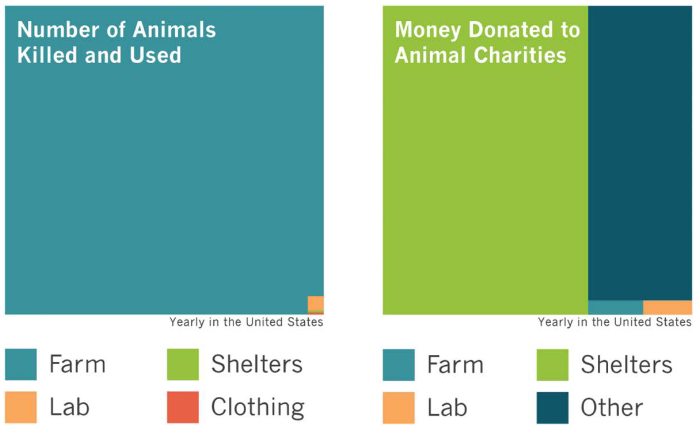
\includegraphics[width=0.5\textwidth, trim={0 2cm 0 0}]{static/assets/img/figure}
    \label{fig:figure2}
\end{figure}
‌
\newline
\newline
\\



برای نتایج جستجو در جستجوی تصویر گوگل، تحقیقات ما نشان می‌دهد که حتی یک تغییر جزئی عبارت به شدت بر نتایج جستجوی مفاهیم مشابه مرتبط با حیوانات تأثیر می‌گذارد.
به عنوان مثال، "حیوان مزرعه" و "حیوان پرورشی" ممکن است مفاهیم بسیار مشابهی به نظر برسند، اما آن‌ها نگرش‌های متفاوتی را نسبت به حیوانات نشان می‌دهند.
سازمان \textenglish{\textbf{Sentient Media}} توضیح می‌دهد که «اصطلاح حیوان پرورشی را می‌توان از حیوانات مزرعه متمایز کرد، زیرا دومی نشان می‌دهد که گونه‌های خاصی از حیوانات که معمولاً برای کشاورزی انتخاب می‌شوند، از نظر بیولوژیکی برای مصرف انسان طراحی شده‌اند».
پیشنهاد علاوه بر این، به نظر می‌رسد کلمه "مزرعه" مفهوم کلی خوبی دارد.
هنگامی که "حیوان مزرعه" جستجو شد، نتیجه برتر و بیشتر (76) از 100 نتیجه برتر، حیوانات کارتونی در مراتع یا انبارهای سبز، دنج، باز و با برخی از حیوانات با "چهره های خندان" هستند (جدول صفحه‌ی بعد).
هنگامی که "حیوانات پرورشی" جستجو شد، اگرچه نتیجه برتر همچنان یک کارتون بود، تنها 6 نتیجه از 100 نتیجه برتر حیوانات کارتونی بودند.
الگوی مشابهی هنگام مقایسه نتایج جستجوی "مزرعه کارخانه" و "کشاورزی حیوانات" یافت شد.
کلمات خنثی تر "کشاورزی حیوانات" نتایج خنثی‌تری را به همراه داشت.
نتایج جستجوی «حیوانات مزرعه» و «کشاورزی حیوانات» نماینده درصد واقعی حیوانات پرورشی که در موقعیت‌های شلوغ زندگی می‌کنند نیست.
بر اساس گزارش موسسه \textenglish{\textbf{Sentience}}، 99 درصد از حیوانات پرورشی زمینی در "مزرعه‌های کارخانه‌ای" زندگی می‌کنند، اصطلاحی که آن‌ها و بسیاری از حامیان حیوانات پرورشی برای توصیف "عملیات تغذیه متمرکز حیوانات" استفاده می‌کنند، اصطلاحی که توسط وزارت کشاورزی ایالات متحده استفاده می‌شود.
و آژانس حفاظت از محیط زیست ایالات متحده از سوی دیگر، انجمن آمریکایی برای پیشگیری از ظلم به حیوانات تخمین می‌زند که «95 درصد حیوانات مزرعه در ایالات متحده در مزارع کارخانه‌ای پرورش می‌یابند».




\begin{figure}
    \centering
    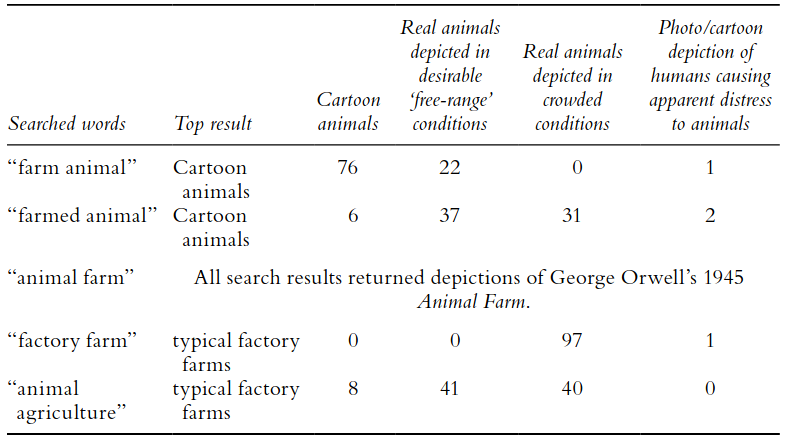
\includegraphics[width=1\textwidth, trim={0 2cm 0 0}]{static/assets/img/figure2}
    \label{}
\end{figure}
‌
\newline
\newline



{\setstretch{0.5}
\phantomsection
\section*{هوش مصنوعی در کشاورزی کارخانه‌ای}
\label{sec:هوش مصنوعی در کشاورزی کارخانه‌ای}
\addcontentsline{toc}{section}{هوش مصنوعی در کشاورزی کارخانه‌ای}{\protect\numberline{}}
اگر سوگیری الگوریتمی گونه‌گرا بر حیوانات غیرانسانی به طور غیرمستقیم با تأثیر بر نگرش انسان نسبت به آن‌ها تأثیر می‌گذارد، برخی دیگر از سیستم‌های هوش‌مصنوعی و کاربردهای علم‌داده به طور مستقیم بر زندگی حیوانات تأثیر می‌گذارند. استفاده از هوش‌مصنوعی و علم‌داده در کشاورزی‌کارخانه‌ای نمونه است.
}

با حسگرهای بیومتریک و حسگرهای محیطی، می‌توان داده‌های زیادی را از حیوانات پرورشی جمع‌آوری کرد و انواع تشخیص و پیش‌بینی الگو را انجام داد.
این‌ها فرصت‌های سودآور جدیدی مانند کاهش‌هزینه، کاهش‌ریسک (احتمال کمتر برای حوادث مرگ و میر بالا یا \textenglish{\textbf{100\%}}) یا محصولات غذایی با کیفیت بالاتر را فراهم می‌کنند.

در سال‌های اخیر، چنین سیستم‌های داده‌محور شروع به آزمایش یا استفاده در صنعت کشاورزی کارخانه‌ای کرده‌اند.
این سیستم‌ها می‌توانند داده‌های حیوانات پرورشی مانند دمای بدن، صداها، وزن، سرعت رشد و مشکلات قابل مشاهده سلامتی مانند جراحات، کبودی ها و انگل‌ها را جمع‌آوری کنند.
مدل‌های یادگیری‌ماشین برای مرتبط کردن پارامترهای‌فیزیکی با معیارهای مهم سودآوری، مانند بیماری، مرگ و میر، نرخ رشد، الگوهای غذا خوردن و غیره ایجاد می‌شوند.
این سیستم‌ها می‌توانند توصیه‌هایی ارائه دهند، یا حتی گاهی اوقات اقدامات مستقیمی را از طریق روباتیک انجام دهند، مانند تغییر مقدار غذای ارائه شده، درمان بیماری، یا حذف.

در پرورش ماهی در سیستم‌های بسته، دو منبع عمده خطرات و هزینه‌ها بیماری‌ها و کم یا بیش از حد تغذیه است.
اولی بر میزان مرگ و میر و کیفیت محصول تأثیر می‌گذارد، در حالی که دومی بر نرخ رشد (کم تغذیه) یا هزینه‌ی خوراک مصرف شده، کیفیت آب و آلودگی (تغذیه بیش از حد) تأثیر می‌گذارد.
مدل سنتی برای مقابله با این دو مشکل، تجربه، شهود و شانس است.
اگرچه برخی از مکانیسم‌های آموزش و گسترش دانش در صنعت وجود دارد، هنوز هم می‌توان گفت که هر پزشک مدل‌های منحصر به فرد خود را دارد.

اما شیوه جدیدی از کار در این صنعت در سال‌های اخیر پدیدار شده است.
برخی از شرکت‌های خدمات آبزی پروری مانند \textenglish{\textbf{Aquabyte}} با شرکت‌های آبزی پروری کار می‌کنند تا به آن‌ها اجازه دهند از ابزارهای \textenglish{\textbf{Aquabyte}}، رابط برنامه‌نویسی، کامپیوترهای تخصصی و مهم‌تر از همه، مدل‌های یادگیری‌ماشین استفاده کنند که همه یادگیری، مدل‌سازی و تصمیم‌گیری مهم را انجام می‌دهند.
به عنوان مثال، شپش دریایی، یک انگل خارج از پوست، اغلب بر روی پوست ماهی قزل آلا دیده می‌شود و یک مشکل رایج برای صنعت پرورش ماهی آزاد در سطح جهان است.
با توجه به خطر انتشار شپش دریایی از ماهی آزاد پرورشی به ماهی قزل آلا وحشی و سایر حیوانات آبزی، حوزه‌های قضایی مختلف نیاز به نظارت و کنترل دقیق سطح شپش دریایی برای تأسیسات پرورش ماهی آزاد دارند.
روش سنتی برای نظارت بر شپش دریایی، برداشتن نمونه‌ای از ماهی قزل‌آلا و شمارش واقعی شپش‌های دریایی است.
\textenglish{\textbf{Aquabyte}} از تکنیک‌های تشخیص تصویر رایانه‌ای برای شمارش تعداد شپش‌های دریایی روی هر ماهی آزاد از تصاویر گرفته شده در زیر آب استفاده می‌کند، که نه تنها کار را کاهش می‌دهد، بلکه نیازی به خارج کردن ماهی آزاد از آب نیست (اقدامی که به سلامت آن‌ها آسیب می‌زند).
الگوریتم تشخیص تصویر با استفاده از داده‌های تأیید‌شده توسط انسان برای گسترش مجموعه‌ی داده آموزشی که الگوریتم بر اساس آن است، بهبود می‌یابد.
علاوه بر شپش دریایی، مشکل تغذیه کم یا بیش از حد نیز می‌تواند با استفاده از داده‌ها و یادگیری‌ماشین حل‌شود.
\textenglish{\textbf{Umitron}}، رقیب \textenglish{\textbf{Aquabyte}}، از الگوریتم‌های یادگیری‌ماشین برای تجزیه و تحلیل داده‌های ویدئویی برای محاسبه اشتهای ماهی بر حسب شاخص استفاده می‌کند.
این الگوریتم "رفتار ماهی خواری را همراه با شرایط مشاهده می کند، قبل از اینکه اشتهای آنها را به ثمر برساند و داده‌ها را در نموداری قابل‌درک ارائه دهد." آن‌ها ادعا می‌کنند که "این به کشاورزان اجازه می‌دهد تا هنگام تغذیه ماهی‌های خود تصمیمات مبتنی بر داده اتخاذ کنند".

همچنین می‌توان از یادگیری‌ماشین برای آموزش الگوریتم‌هایی برای «شناسایی» وضعیت رفاه حیوانات (هم حیوانات همراه و هم حیوانات پرورشی داده‌شده در کارخانه استفاده کرد).
طبق تحقیقات ما یک مشکل مشترک با الگوریتم‌هایی وجود دارد که مدعی شناسایی وضعیت‌های رفاهی/رفتاری در حیوانات هستند.
همه داده‌هایی که برای آموزش الگوریتم‌ها استفاده می‌شوند توسط انسان‌ها برچسب‌گذاری می‌شوند و در نتیجه توسط ارزش‌ها و قضاوت‌های تجربی خود ما سنگینی می‌کنند تا اینکه دقیقاً منعکس‌کننده علایق خود حیوان و تعیین‌های ذهنی از آنچه خود حیوان برای آن ارزش قائل است.
بنابراین دقت و قابل اعتماد بودن الگوریتم‌ها به این محدود می‌شود که ما انسان‌ها در وهله اول تا چه حد در رمزگشایی زندگی ذهنی حیوانات قابل اعتماد و دقیق بوده‌ایم.
تحقیقات بیشتر در مورد اینکه چگونه حیوانات می‌توانند با استفاده از سیستم‌های هوش‌مصنوعی برچسب‌گذاری کنند و رفاه خود را ارتقا دهند، به فوریت مورد نیاز است.
اما برای جلوگیری از تعصب، باید توسط افرادی انجام شود که ذینفعان صنعت کشاورزی کارخانه نیستند.
\newline
\newline



{\setstretch{0.5}
\phantomsection
\section*{تفسیر}
\label{sec:تفسیر}
\addcontentsline{toc}{section}{تفسیر}{\protect\numberline{}}


\phantomsection
\subsection*{اخلاق یهود}
\label{subsec:اخلاق یهود}
\addcontentsline{toc}{subsection}{اخلاق یهود}{\protect\numberline{}}
\noindent \textbf{نوشته دانیل سینکلر}
\\\\
دو اصل اساسی کتاب مقدس حاکم بر رویکرد سنتی یهودیان به حیوانات، تسلط انسان بر سایر موجودات زنده است که در برکت خداوند برای آدم و حوا ذکر شده است:«و بر ماهیان دریا و بر مرغان آسمان تسلط داشته‌باشید، و بر هر حیوانی که روی زمین ازدحام می کند».
و منع ایجاد رنج برای هر موجود زنده‌ای در حین اعمال آن سلطه.
}

میمونیدس شتاب و عصبانیت بالا بلاعم را به خاطر ضرب و جرح سختی که به خر خود وارد کرد، به عنوان منبعی برای تحریم این کار تشخیص می‌دهد.
مراجع دیگر منبع آن را در قوانین مختلف از جمله الزام به کمک به تخلیه‌ی حیوانی که زیر بار خود فرورفته است و ممنوعیت پوزه زدن گاو هنگام خرمن کوبی می‌دانند.
نکته قابل توجه این است که طبق قوانین کتاب مقدس، حیوانات نیز باید در روز استراحت کنند و باید به چراگاه دسترسی داشته‌باشند تا نه تنها از کار رها شوند، بلکه رضایت و خشنودی نیز فراهم شود.
علاوه بر این، تلمود حکم می‌کند که در موارد خاص، حفظ رفاه حیوانات بر ممنوعیت‌های روز مقدس غلبه می‌کند.

اصل سلطه‌ی استفاده از حیوانات را برای طیف وسیعی از نیازهای انسان از جمله غذا توجیه می‌کند.
با این حال، در آغاز، انسان‌ها گیاه‌خوار بودند و اجازه مصرف گوشت حیوانات تنها در دوران پس از غرق شدن با این قید داده می‌شد که حیوان قبل از مصرف آن ذبح شود.
بر اساس یک دیدگاه، دلیل این امتیاز این بود که نوع بشر پس از سیل از نظر جسمی انحطاط پیدا کرد و در نتیجه مردم دیگر قادر به تامین نیازهای غذایی خود نبودند مگر اینکه گوشت بخورند.
توضیح دیگری برای تغییری که «آرکوک» \textenglish{\textbf{(1865-1935)}} در تک‌نگاری خود ("چشم انداز گیاه‌خواری و صلح") ارائه کرد، سطح بسیار پایین اخلاق و معنویت در دوره پساغذایی است که خود را در شهوت ظاهری نشان داد.
گوشت به منظور جلوگیری از آدم‌خواری، انسان‌ها مجاز به خوردن گوشت حیوانات بودند، اما نه از نوع خود.
آرکوک مشتاقانه منتظر عصری است که در آن بشر از نظر اخلاقی تا حدی تکامل یابد که این تصور را که مجاز بودن مصرف گوشت هر موجود زنده‌ای مجاز است، کاملاً رد کند.
با این حال، در این میان، حیوانات ممکن است برای گوشتشان ذبح شوند، اما همانطور که میمونیدس اشاره می‌کند، کشتار باید تا حد امکان بدون درد انجام شود.
از این رو، انبوهی از مقررات حاکم بر ذبح آیینی در قوانین یهود، که هدف آن‌ها تضمین حداقل رنج حیوانات در این فرآیند است.

پرهیز از ظلم نه تنها انگیزه قوانین ذبح آیینی است، همچنین به عنوان یک محدودیت اخلاقی فراقانونی در استفاده از حیوانات برای گوشت عمل می‌کند.
تلمود نقل می‌کند که «آرجودا» شاهزاده، ویرایشگر میشنا، در حال سخنرانی عمومی بود که گوساله‌ای که به کشتارگاه هدایت می‌شد، وارد سالن شد و سر خود را زیر گوشه ردای خود فرو کرد و با ترحم پایین انداخت.
«آرجودا» به گوساله گفت: «برو!
شما برای این منظور آفریده شده‌اید [که ذبح شوید]».
در آن لحظه در بهشت گفته شد: «چون او رحم نکرد، بگذار رنج ببرد» و سیزده سال به بیماری دردناکی مبتلا بود.
یک روز، خدمتکار او در حال جارو کردن خانه بود که به زباله‌هایی از راسوهای تازه متولد شده برخورد کرد و می‌خواست آن‌ها را جارو کند که «آرجودا» گفت: «بگذارید آن‌ها باشند.
چنانکه نوشته شده است: «وَ أَرْحَمْتَهُ عَلَیْهَهُ عَلَیْهِهِ» در بهشت گفتند: «چون او رحمت می‌کند، به او رحم کنیم» و دردش قطع شد.
به گفته مفسران تلمودی، «آرجودا» به این دلیل مجازات شد که در نقش خود به عنوان رهبر نسل خود، مسئولیت او این بود که با ابراز همدلی و نجات گوساله، شنوندگان خود را به اصل فراقانونی جلوگیری از ظلم آموزش دهد.
در شرایط خاص پرونده، استناد به قانون قابل‌قبول نبود.

دامپروری معاصر باعث ایجاد انبوهی از چالش‌های اخلاقی فراتر از کشتار بدون درد و استفاده‌های سنتی از دام شده است.
فناوری، از جمله هوش‌مصنوعی، زندگی حیوانات را از بدو تولد تا مرگ کنترل می‌کند و به ویژه در پنهان کردن ظلمی که اغلب در دامپروری مدرن انجام می‌شود، ماهر است.
یکی از ابتکارات اصلاح‌کننده یهودیان در این زمینه، پروژه «ماگن تزِدک» در سال 2011 جنبش محافظه‌کار است که به دنبال برچسب زدن به غذای «اخلاقی به‌دست‌آمده» است، علاوه بر برچسب معروف‌تر کوشر (هخشر) که نشان‌دهنده‌ی مناسب بودن آیینی آن است.
\newline
\newline



{\setstretch{0.5}
\phantomsection
\subsection*{اخلاق دئونتولوژیک}
\label{subsec:اخلاق دئونتولوژیک}
\addcontentsline{toc}{subsection}{اخلاق دئونتولوژیک}{\protect\numberline{}}
\noindent \textbf{نوشته کالین مارشال}
\\\\
همانطور که در مورد "حیوانات و هوش‌مصنوعی غیرانسان" توضیح داده شده‌است، هوش‌مصنوعی و فناوری‌های مرتبط تاثیر زیادی بر حیوانات و نگرش ما نسبت به آن‌ها دارند، در مقیاسی که چند‌دهه پیش غیرقابل تصور بود.
}

همه‌ی نسخه‌های دئونتولوژیک موافق هستند که ما برخی تعهدات اخلاقی در رابطه با حیوانات داریم.
با این حال، برخی از نسخه‌های دئونتولوژیک معتقدند که حیوانات از نظر اخلاقی مانند انسان‌ها مهم هستند، در حالی که نسخه‌های دیگر معتقدند که اهمیت اخلاقی آن‌ها از نوع کمتر و متفاوت است.
ما می‌توانیم این مورد را از هرمنظری به نوبه‌ی خود بررسی کنیم.

اگر حیوانات از نظر اخلاقی مانند انسان‌ها مهم هستند، پس دئونتولوژی به این معنی است که آن‌ها نیز شایسته‌ی احترام اخلاقی هستند.
برای دندان شناسان، یکی از مؤلفه‌های کلیدی احترام اخلاقی این است که نیازها و پروژه‌های دیگران را جدی بگیریم، و آن‌ها را در تعقیب اهداف خود زیر پا نگذاریم (یعنی استفاده از آن‌ها به عنوان وسیله‌ای صرف).
این که در موارد خاص به چه چیزی تبدیل می‌شود بستگی به نیازها و پروژه هایی دارد: خندیدن به بداخلاقی‌های یک کمدین می‌تواند کاملا محترمانه باشد، اما خندیدن به صدمات جسمی فرد دیگر می‌تواند عمیقاً بی‌احترامی باشد (جدی نگرفتن نیازهای فیزیکی آن‌ها و استفاده از آن‌ها به عنوان وسیله‌ای صرف برای سرگرمی).

بسیاری از اشکال سوگیری شامل عدم‌رعایت احترام است.
به عنوان مثال، تعصب نژادی سیستماتیک می‌تواند شامل ناتوانی اعضای یک نژاد در مورد جدی گرفتن نیازها و پروژه‌های نژادهای دیگر باشد و استفاده از نژاد دوم را به عنوان وسیله‌ای ساده برای نژادهای دیگر آسان‌تر می‌کند.
سوگیری‌های الگوریتمی در موتورهای جستجو می‌تواند این گونه شکست‌های احترام را تداوم و تقویت کند.
زمانی که جستجو برای «حیوان آزاری» و «حفاظت از حیوانات» به طور گمراه‌کننده نتایج بسیار بیشتری را در رابطه با سگ‌ها نسبت به سایر گونه‌ها نشان می‌دهد، این خود ناتوانی در جدی گرفتن نیازهای گونه‌های دیگر است و می‌تواند باعث تداوم ناکامی‌های موجود در احترام در افرادی شود که از جستجو استفاده می‌کنند.
موتور چنین شکست‌هایی باعث می‌شود که افراد برای دستیابی به اهداف خود، اغلب سطحی، مانند لذت‌های آشپزی، حیوانات دیگر را (گاهی به معنای واقعی کلمه) زیر پا بگذارند.
به طور مشابه، فن‌آوری‌های افزایش کارآیی که در کشاورزی کارخانه‌ای مورد استفاده قرار می‌گیرند، می‌توانند شامل و تداوم شکست‌های احترام شوند، به جای اینکه حیوانات را به‌عنوان موجوداتی که نیازهایشان مورد توجه قرار می‌گیرد، صرفاً به‌عنوان نقاط داده‌ای در یک فرآیند سودآور رفتار کنند.

اما اگر انکار کنیم که حیوانات از نظر اخلاقی مانند انسان ها مهم هستند، چه؟ دئونتولوژیست‌هایی که این ادعا را رد می‌کنند، می‌توانند این گونه درک شوند که می‌گویند شکل خاصی از گونه‌گرایی (یا چیزی نزدیک به آن) قابل دفاع است، اغلب به دلیل تفاوت در عقلانیت بین انسان‌ها و گونه‌های دیگر.
با این وجود، دین شناسان در این سنت استدلال کرده‌اند که احترامی که ما به انسان‌ها مدیونیم، باعث ایجاد تعهدات نسبت به حیوانات می‌شود.
دلیل این امر این است که انسان‌ها دارای ویژگی‌های بسیاری با سایر حیوانات هستند، مانند نیاز ما به تغذیه، انگیزه برای تولید مثل و ظرفیت برای درد و لذت.
به همین دلیل، تمایل به سوء‌استفاده یا نادیده گرفتن منافع حیوانات به راحتی می‌تواند منجر به عدم احترام به انسان شود یا حتی ممکن است به خودی خود منجر شود.
تصور کنید کودک کوچکی را ببینید که با خوشحالی با یک چاقوی اسباب‌بازی به صورت یک حیوان عروسکی می‌کوبد.
حتی با وجود اینکه هیچ آسیب واقعی وارد نشده‌است، ممکن است به طور منطقی عمل را به دلیل بی اعتنایی به رنج نشان می‌دهد، ذاتاً قابل اعتراض بدانیم، و ممکن است نگران باشیم که چه آسیب‌های واقعی ممکن است منجر شود.

بی تفاوتی در مقیاس بزرگ به نیازهای، به عنوان مثال، حیوانات زمینی وحشی و باله‌ماهی‌ها را در نظر بگیرید که توسط فناوری‌های شرح داده‌شده در فصل ترویج می‌شوند.
این بی‌تفاوتی، جدی نگرفتن مرگ و رنج تعداد زیادی از موجودات زنده است.
حتی اگر آن موجودات از نظر اخلاقی کمتر از انسان‌ها اهمیت داشته‌باشند، این بی‌تفاوتی شبیه بی‌تفاوتی نسبت به رنج‌های بزرگ انسانی، مانند قحطی در کشورهای جهان سوم است.
حفاظت از احترام شکننده‌ای که برای سایر انسان‌ها داریم یا باید داشته‌باشیم، مسلماً مستلزم توجه جدی‌تر به نیازهای حیوانات است.

دو خط فکری شرح داده‌شده در این تفسیر با هم سازگارند.
می‌توان هم معتقد بود که حیوانات به خودی خود سزاوار احترام اخلاقی هستند و هم اینکه ما باید نگرش خود را نسبت به آن‌ها تنظیم کنیم تا از احترامی که به انسان‌های دیگر مدیونیم حمایت کنیم.
در هر دو رویکرد، دئونتولوژیک حداقل می‌خواهد که توسعه‌دهندگان فناوری نیازهای حیوانات را پنهان نکنند.
پاسخگویی کامل به حداقل تقاضا نیازمند تغییرات قابل توجهی در پلتفرم‌های موجود است، اما بسیاری از پاسخ‌های مقیاس کوچکتر در دسترس هستند.
\newline
\newline



{\setstretch{0.5}
\phantomsection
\subsection*{اخلاق آفریقایی}
\label{subsec:اخلاق آفریقایی}
\addcontentsline{toc}{subsection}{اخلاق آفریقایی}{\protect\numberline{}}
\noindent \textbf{نوشته جان مورانگی}
\\\\
درخواست برای به رسمیت شناختن حقوق اخلاقی حیوانات توسط تعداد فزاینده‌ای از اخلاق شناسان مطرح می‌شود. با این حال، مانعی که آن‌ها به دنبال غلبه بر آن هستند توسط کسانی ایجاد شده است که حقوق بشر را محدود کرده‌اند. آن‌ها این محدودیت را پیش‌داوری گونه‌ای می‌دانند که به موجب آن انسان‌ها خود را دارندگان انحصاری این حقوق می‌دانند. از نظر آن‌ها، هر موجودی که در معرض رنج است، مستحق مالکیت ذاتی این حقوق است. از آنجایی که حیوانات رنج می‌برند، شایسته است که در میان دارندگان این حقوق قرار گیرند.
}

یک دیدگاه جامع از هوش‌مصنوعی باید ماهیت فناوری را در‌نظر بگیرد.
این ممکن است برای بسیاری از تولیدکنندگان، صاحبان، مدیران و کاربران فناوری آشکار باشد، اما آنچه بدیهی به نظر می‌رسد ممکن است اینطور نباشد.
سؤال در مورد ماهیت فناوری اساساً مطرح نشده‌است و تا این حد نحوه عملکرد هوش‌مصنوعی در رابطه با فناوری ناگفته باقی‌مانده است.
در نتیجه، یکی از خطرات این است که ماهیت هوش‌مصنوعی نادیده گرفته‌می‌شود.
خود اندیشیدن به یک موضوع فناوری تبدیل شده است.
تفکر فنی شده‌است.
موضوع هوش‌مصنوعی است.
هوش‌مصنوعی و فناوری (مادر آن) به طور فزاینده ای تنها تعیین کننده چیستی تفکر شده‌اند.
اشتراک فکری توسط هوش‌مصنوعی به طور فزاینده‌ای به واقعیت زمان ما تبدیل شده‌است.
هوش‌مصنوعی در تعیین ماهیت تفکر به طور فزاینده‌ای دیکتاتوری شده‌است.
تمایز بین آنچه واقعی و مصنوعی است به قدری مبهم بوده است که واقعی تبدیل به مصنوعی شده است.
این بر ادعاهای مربوط به محل و صاحبان حقوق اخلاقی تأثیر می‌گذارد.

«مارتین هایدگر، فیلسوف بزرگ آلمانی قرن بیستم» سهم مهمی دارد.
او می‌گوید:

\begin{quote}
    ماهیت تکنولوژی به هیچ وجه هیچ چیز تکنولوژیکی نیست.
    بنابراین، ما هرگز رابطه‌ی خود را با ذات فناوری تجربه نخواهیم کرد تا زمانی که صرفاً فناوری را تصور کرده و به جلو می‌بریم، آن را تحمل می‌کنیم یا از آن طفره می‌رویم.
    در همه جا ما غیرآزاد و به زنجیر تکنولوژی می‌مانیم، چه با شور و شوق آن را تأیید کنیم و چه آن را انکار کنیم.
    اما زمانی که آن را چیزی خنثی می‌دانیم، در بدترین حالت به آن تحویل می‌شویم، زیرا این تصور از آن، که امروزه به‌ویژه دوست داریم به آن ادای احترام کنیم، ما را نسبت به ماهیت فناوری کاملاً کور می‌کند.
    \\\\
    \newline
    \newline
\end{quote}

هایدگر به ما یادآوری می‌کند که هیچ چیز تکنولوژیکی در مورد ماهیت فناوری وجود ندارد.
بدون پرداختن به جزئیات در مورد درک او از ماهیت فناوری، به نظر می‌رسد که فناوری آرم تکنو، انسان شناسی است.
یعنی آرم آنتروپوس است.
در اینجا ما نباید انسان شناسی را به عنوان رشته ای که در آکادمی تدریس می‌شود در نظر بگیریم.
ما باید مطالعه‌ای داشته‌باشیم که انسان بودن چیست و چه چیزی در سعادت انسان در خطر است.

اکثراً، این دیدگاه که در نهایت فناوری انسان‌شناسی است، به ندرت توسط کسانی که درگیر آن هستند مورد توجه قرار می‌گیرد.
این مورد در مورد کسانی است که خود را معرفی می‌کنند یا کسانی که به عنوان دانش آموزان هوش‌مصنوعی یا به طور کلی به عنوان دانشجویان فناوری معرفی می‌شوند.
آن‌ها این مطالعه را به عنوان مطالعه در مورد اینکه چه کسی یا چه چیزی هستند و در نهایت چه چیزی باعث رفاه ما می‌شود، نمی‌گیرند.
آن‌ها خود را فرزندان هوش‌مصنوعی یا مادر و پدر هوش‌مصنوعی نمی‌دانند.

با فرض اینکه تکنولوژی انسان‌شناسی است، این انسان‌شناسی به شدت مشکل ساز است.
در مدرنیته اروپایی، «گئورگ ویلهلم فردریش هگل، فیلسوف برجسته آلمانی»، ادعا کرد که:

\begin{quote}
    سیاه پوست، همانطور که قبلاً مشاهده شد، انسان طبیعی را در حالت کاملاً وحشی و رام نشده خود به نمایش می‌گذارد.
    اگر بخواهیم او را به درستی درک کنیم، تمام فکر احترام و اخلاق را کنار می‌گذاریم (همه‌ی آنچه را احساس می‌نامیم).
    هیچ چیز هماهنگ با انسانیت در این نوع شخصیت یافت نمی‌شود.
    \\\\
    \newline
    \newline
\end{quote}

سخنان «هگل، ژان پل سارتر، فیلسوف فرانسوی»، سخنانی را درباره یهودی ستیز به ذهن متبادر می‌کند.
سارتر استدلال می‌کند که برای یهودستیز، یهودی‌ای که یهودی‌ستیز است، اساساً شرور است، اختراع ذهن اوست.
اگر یهودی وجود نداشت، باید یکی را اختراع می‌کرد.
یهودی‌ستیز می‌خواهد از خود پنهان کند که یهودی مورد نظر او اختراع ذهن اوست و از این حقیقت پنهان می‌ماند زیرا پذیرش آن وابستگی مطلق او به یهودی را برای وجودش آشکار می‌کند.
به طور مشابه، آنچه هگل به عنوان یک سیاه‌پوست می‌گیرد چیزی بیش از اختراع ذهن او نیست.
در اختراع سیاه‌پوست، خودش را اختراع می‌کند.
هیچ سیاه‌پوستی جز در ذهن هگل و در ذهن کسانی که مانند او می‌اندیشند وجود ندارد.
آفریقایی ها آفریقایی هستند.
آنها سیاه پوست نیستند.
برای آفریقایی‌ها، سیاه پوستان آفریقایی نیستند.

باید واضح باشد که قلمروی هوش‌مصنوعی قلمرو اختراع است.
ظاهراً اینجا به یک قلمرو فضای مجازی تبدیل شده است.
بحث اخلاق به یک سؤال فضای مجازی تبدیل شده است.
یکی از جنبه‌های این پرسش این است که چه کسی در این حوزه اخلاقاً حکومت می‌کند و به نفع چه کسی است؟ آیا حیوانات اینجا حرفی برای گفتن دارند؟ اینجا جایی است که روایت هگل از اومانیسم مرتبط است.
از آنجایی که او آفریقایی‌ها را از جامعه انسان‌ها کنار می‌گذارد، به نظر می‌رسد که آفریقایی‌ها چیزی برای کمک به حاکمیت اخلاقی فضای مجازی یا تعیین اینکه چه کسی یا چه کسی حقوق اخلاقی دارد، ندارند.

در نظر داشته‌باشیم که فضای‌مجازی فضایی است کاملاً بریده از فضای زمینی.
مدرنیته اروپایی نسخه خاص خود از استعمار را ابداع کرده است.
آیا ممکن است فضای‌مجازی یک فضای استعمار شده باشد و در حال گذراندن فرآیند استعمار باشد و هوش‌مصنوعی عامل اصلی این فرآیند باشد؟

به نظر من آنچه آفریقایی‌ها می‌توانند به بحث اخلاق در عصر فضای مجازی کمک کنند، یک اخلاق آزادی‌بخش است (اخلاقی که سلاح‌های ظالمانه‌ی هوش‌مصنوعی را به رسمیت می‌شناسد).
استفاده از هوش‌مصنوعی برای رهایی نوع بشر از نظر اخلاقی قابل‌توجه است و می‌تواند راهی برای رهایی حیوانات بگشاید.
با وجدان خوب، ما نمی‌توانیم حیوانات را به‌عنوان حاملان حقوق اخلاقی بشناسیم، اگر درک کافی از کیستی یا چیستی خود نداشته‌باشیم.

یکی از مفاهیم کلیدی در اخلاق آفریقا اوبونتو است.
ادعای اصلی در این اخلاق این است که ما هستیم پس من هستم.
«ما» چیزی بیش از مجموع «هست» است.
یک «ما» جمعی است.
در این اخلاق، آنچه باقی می‌ماند این است که چه کسانی در آن گنجانده شده یا حذف شده‌اند.
هنوز جای این حیوان مشخص نشده است.
تا جایی که فکر نشود، انسان باقی می‌ماند تا فکر شود.
بر این اساس، جنبه اخلاقی «ما» باید به طور کامل بررسی شود.
حاکمیت هوش‌مصنوعی امروز مانع بزرگی برای ظهور این تفکر است.
انسان شناسی سایبری (انسان سایبری به عنوان یک مانع بزرگ در راه است).



